\chapter{Selecci\'on de contenido de expresiones referenciales}
\label{sec:seleccion}

Una propiedad es una caracter\'istica de un objeto. Una relaci\'on es otra caracter\'istica la cual incluye a otro u otros objetos.\\

La selecci\'on de cuales propiedades y/o relaciones con otros objetos incluir en una expresi\'on referencial depender\'a del prop\'osito que tengamos para dicha expresi\'on referencial, claramente ser\'a muy distinta la expresi\'on si nuestro objetivo es dar la m\'inima expresi\'on referencial que identifique al objeto que si nuestro objetivo es ser colaborativos con nuestro interlocutor.\\

En la vida real hay muchas cosas que nos ayudan a darnos cuenta si nuestro interlocutor identific\'o el objeto target, como ser la expresi\'on de sorpresa nos dar\'ia una pauta de que no esta entendiendo lo que le queremos decir, pero cuando queremos hacer esa generaci\'on autom\'atica normalmente no poseemos esa clase de informaci\'on.\\

En esta tesis nos vamos a enfocar en la selecci\'on de contenidos de las expresiones referenciales, y el objetivo ser\'ia simular el comportamiento humano, para ello vamos a usar corpus de expresiones referenciales para aprender como realizan esta tarea las personas.\\

En este Cap\'itulo daremos una introducci\'on a la generaci\'on autom\'atica de expresiones referenciales, las propiedades que puede tener o no una expresi\'on referencial y los algoritmos para generarlas, y luego explicaremos los algoritmos m\'as conocidos en el \'area.


\section{Propiedades de una ER}

%Cuando la ER no es relacional solo contiene propiedades del objeto mismo. Ej.: color, tama\~no. Note que quiz\'as el tama\~no sea con respecto a los dem\'as objetos ``la m\'as peque\~na'', pero al no incluir una descripci\'on de otro objeto no la llamamos relacional.\\
Una ER puede ser relacional o no relacional (tambi\'en llamada proposicional), minimal o sobreespecificada, y subespecificada en cuyo caso es una expresi\'on que no es referencial, la incluimos en nuestras propiedades porque nos va a ser \'util la defici\'on en el Cap\'itulo \ref{sec:corpus}.\\

Una ER es {\it relacional}, cuando contiene relaciones con otros objetos, entonces aqu\'{i} se incluye en desaf\'{i}o de describir al siguiente objeto. Ej.: ``La que esta al lado del cubo rojo''. En este caso, ``al lado del'' es una relaci\'on entre el objeto target y otro objeto cuya ER es el ``cubo rojo''.\\

Una ER {\it proposicional} incluye solo propiedades absolutas del objeto target. Ej.: ``La pelota roja con rayas amarillas''. Las caracter\'isticas ser pelota, roja y tener rayas amarillas son propias del objeto a identificar.\\

Se dice que una ER es {\it minimal}, cuando incluye la m\'inima cantidad de propiedades con la cual puede ser identificada un\'ivocamente en el contexto dado. Notar que puede haber muchas expresiones minimales.\\

En cambio cuando contiene m\'as informaci\'on de la m\'inima necesaria para identificarla un\'ivocamente de los dem\'as objetos en el contexto dado, se dice que la ER es {\it sobreespecificada}.\\

{\it Subespecificada} es cuando la expresi\'on dada, no alcanza a ser una ER, ya que no se puede identificar al objeto target del resto de los objetos en la imagen. En estos casos se debe dar otra expresi\'on o corregir la anterior agregando m\'as propiedades o relaciones. Esta expresi\'on identifica a un conjunto, no a un objeto \'unico.


\section{Propiedades de un algoritmo}

En esta parte definiremos el problema en general, cuando queremos generar las ER autom\'aticamente simulando lo encontrado en un corpus, en un corpus tenemos ER dadas por muchas personas. Los algoritmos para generarlas pueden tener algunas de las siguientes propiedades.\\

Un algoritmo puede ser: determin\'{i}stico o no-determin\'{i}stico, relacional o proposicional, incluir negaciones o no, identificar plurales o solo singulares, usar disyunciones adem\'as de conjunciones, o solo conjunciones, generar ER sobreespecificadas o minimales. Hacer o no backtraking.\\

Un algoritmo es {\it determin\'{i}stico} si dado un input (una escena, con un objeto target), da siempre la misma ER de salida. En cambio es {\it no-determin\'{i}stico} si considera la posibilidad de dar distintas salidas para el mismo input, en distintas ejecusiones simulando el comportamiento de distintas personas, o incluso el de la misma persona en distintos momentos.\\

Un algoritmo es {\it relacional} si permite generar ER relacionales, en cuyo caso adem\'as de generar las relaciones correspondientes deber\'a generar una ER para el objeto con el cual el objeto target tiene la relaci\'on. Notar que las relaciones pueden ser con muchos objetos, es decir de una aridad mayor que 1. Ej.: ``el restaurante que esta en la esquina de Gral. Paz y Col\'on''.\\

En algunos contextos cuando el target es el \'unico que no tiene una propiedad por ejemplo, ser\'ia \'util un algoritmo que incluya {\it negaciones}.\\

Un algoritmo puede generar ER para {\it plurales}, es decir dar ER para varios targets de la escena considerada.\\

Los algoritmos tambi\'en se pueden diferenciar en si usan conjunciones, disyunciones o ambas.\\

La sobreespecificaci\'on es la caracter\'istica de dar m\'as atributos o relaciones de las necesarias para identificar al objeto target. Ser\'ia interesante que un algoritmo diera la sobreespecificaci\'on que las personas dan. Ej.: ``el restaurante que esta en la esquina de Gral. Paz y Col\'on, al frente del correo''.\\

Un algoritmo que hace backtraking, es el que luego de incluir una propiedad o relaci\'on puede deshacer esa inclusi\'on volviendo a un estado anterior, es decir, decidir luego no incluirla.\\

\section{Generaci\'on autom\'atica de expresiones referenciales}

El desaf\'io de la generaci\'on autom\'atica de contenido para las expresiones referenciales viene dado porque una computadora no sabe cuales son las propiedades m\'as sobresalientes de un objetos.

\section{Algoritmos de REG}

Cada objeto o entidad tiene un tipo, ciertas propiedades o caracter\'isticas y los valores de esas propiedades, que incluso pueden ser relaciones con otros objetos. \\

Por ejemplo: Que cosa es? (el tipo) Una pelota. Que color? Rojo. Esta al lado de otro objeto? Si. Cual? El cubo azul.\\

Con esta clase de datos para los objetos de la escena, tenemos una base de conocimento (KB), estos datos se pueden organizar en jerarqu\'ias, por ejemplo: conjunto de animales, conjunto de mamiferos, conjunto de insectos. Algunos conjuntos pueden estar contenidos en otros, es decir algunos objetos o entidades pueden compartir caracter\'isticas.\\

Si tenemos 100 caracter\'isticas de una persona, y con esas caracter\'isticas se pudiera identificar un\'ivocamente a una persona, un sistema que diera que las 100 caracter\'isticas no ser\'ia un sistema que suene muy natural, ya que una persona no dar\'ia 100 propiedades para identicar a una persona particular. As\'i podr\'iamos decir que las expresiones referenciales variaran seg\'un la cantidad de informaci\'on que dan, si dan la m\'inima informaci\'on para identificarlas un\'ivocamente ser\'an minimales, si dan m\'as informaci\'on estar\'an sobreespecificadas, pero en el caso de dar m\'as de la m\'inima informaci\'on... cu\'anta m\'as dar?

El sistema deber\'ia tener una lista del orden de preferencia de los atributos a usar.\\ 

Para una persona identificar ciertos atributos puede ser m\'as f\'acil que identificar ciertos otros, por ejemplo cierto color verde podr\'{i}a ser m\'as complicado de identificar que el tama\~no. Notar que cuando decimos el tama\~no podemos decir ``grande'' y tenemos como marco de referencia a los objetos de la escena, en ese contexto un objeto es ``grande''.\\

Para un algoritmo entonces, ser\'ian cuestiones importantes de tener en cuenta:

\begin{itemize}
 \item Que propiedades o relaciones incluir?
 \item Cuando terminar (dar la expresi\'on minimal? o dar una expresi\'on sobreespecificada, si es sobreespecifica, que tan sobreespecificada?)
 \item Que orden de preferencias seguir?
 \item Hacer o no backtraking?
 \item Incluir o no negaciones?
\end{itemize}



%\subsection{GREEDY}

%Este algoritmo de Dale~\cite{dale89} busca sobre todo el conjunto de propiedades del target y elije el subconjunto m\'as chico posible que identifica un\'{i}vocamente al objeto target entre los distractores en la escena considerada como se muestra en el siguiente algoritmo.\\

%\begin{figure}[ht]
%\begin{center}
%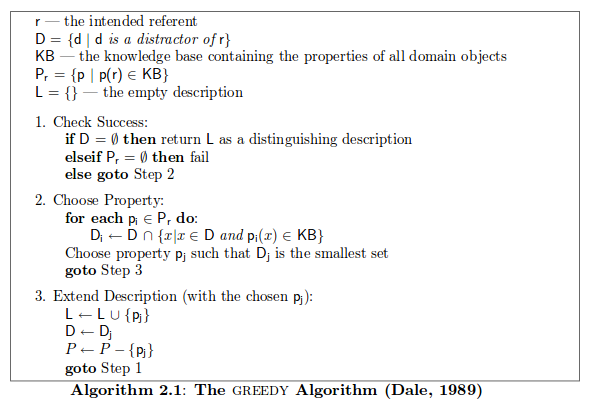
\includegraphics[width=8.5cm]{figures/greedy.png}\\[0pt]
%\caption{Interface del experimento}
%\label{fig-greedy}
%\end{center}
%\end{figure}

%r - el objeto target\\
%D = \{d|d es un distractor de r\}\\
%KB - la base de conocimiento que contiene las propiedades de todos los objetos\\
%$P_{r}$ = $\{p|p(r) \in KB\}$\\
%L = $\{\}$ - la descripci\'on vac\'{i}a\\
%\\
%1. Chequea \'exito:\\
%    \textbf{if} D = $\emptyset$ \textbf{then} return L como una ER que distingue al target r
%    \textbf{elseif} $P_{r}$ = $\emptyset$ \textbf{then} fail
%    
%\textbf{else goto} Paso 2 \\
%\\
%2. Elegir Propiedad:
% \textbf{for each} $p_{i}$ $\in$ $P_{r}$ \textbf{do}:
%    $D_{i}$ $\leftarrow$ D$\cap$ \{x|x $\in$ D and $p_{i}$ (x) $\in$ KB\}
%    Elegir la propiedad $p_{j}$ tal que $D_{j}$ es el conjunto m\'as chico (es decir la que elimina m\'as distractores) \textbf{goto} Paso 3\\
%\\    
%3. Agregar $p_{j}$ a la descripci\'on actual\\
%L $\leftarrow$ L $\cup$ \{$p_{j}$\}\\
%D $\leftarrow$ $D_{j}$\\
%P $\leftarrow$ P -\{$p_{j}$\}\\
%\textbf{goto} Paso 1\\



%%Dado un dominio D que contiene un target referente r y un conjunto de distractores, una base de conocimiento KB que contiene las propiedades de los objetos.
%%Un conjunto de propiedades verdaderas para r, y una descripcion L inicialmente vac\'{i}a.

%Este algoritmo es de orden NP-complete

\subsection{Incremental}

Se describe a continuaci\'on el algoritmo Incremental de Dale \& Reiter el cual reduce la complejidad del algoritmo Greedy (el cual hac\'ia una b\'usqueda exaustiva y elegia la propiedad que m\'as distractores eliminaba en cada paso) cambiando que en vez de chequear cual propiedad es la que elimina m\'as distractores, eligiendo la que sigue en la lista de propiedades ordenada seg\'un preferencia y que posee al menos un distractor. Este algoritmo es de orden polinomial. Este algoritmo produce expresiones referenciales que pueden estar sobreespecificadas.\\

\textcolor{blue}{reescribir esto porque no queda tabulado como un algoritmo}


\fbox{ \begin{minipage}{150mm}

r - el objeto target que queremos identificar\\
D = \{d|d es un distractor de r\}\\
KB - la base de conocimiento que contiene las propiedades de todos los objetos\\
$P_{r}$ = $\{p|p(r) \in KB\}$ ordenado seg\'un preferencia de propiedades\\
L = $\{\}$ - la descripci\'on vac\'{i}a\\

1. Chequea \'exito:\\
    \textbf{if} D = $\emptyset$ \textbf{then} return L como una ER que distingue al target r
    \textbf{elseif} $P_{r}$ = $\emptyset$ \textbf{then} fail\\
\textbf{else goto} Paso 2 \\
\\
2. Seleccionar Propiedad:\\
 \textbf{for each} $p_{i}$ $\in$ $P_{r}$ \textbf{do}:\\
 \textbf{if} \{x|x $\in$ $D_{i}$ and $p_{i}$ (x) $\in$ KB\} $\neq$ $\emptyset$\\
 \textbf{then} elegir $p_{j}$ e \textbf{goto} Paso 3\\
 %(la primer propiedad en el orden que elimima\\ al menos un distractor) 
 
 \textbf{else} $P_{r}$ =$P_{r}$ -$p_{j}$\\
 \textbf{goto} Paso 1\\
      \\    
3. Agregar $p_{j}$ a la descripci\'on actual\\
L $\leftarrow$ L $\cup$ \{$p_{j}$\}\\
D $\leftarrow$ $D_{j}$\\
P $\leftarrow$ P -\{$p_{j}$\}\\
\textbf{goto} Paso 1\\
\end{minipage}}
%\begin{figure}[ht]
%\begin{center}
%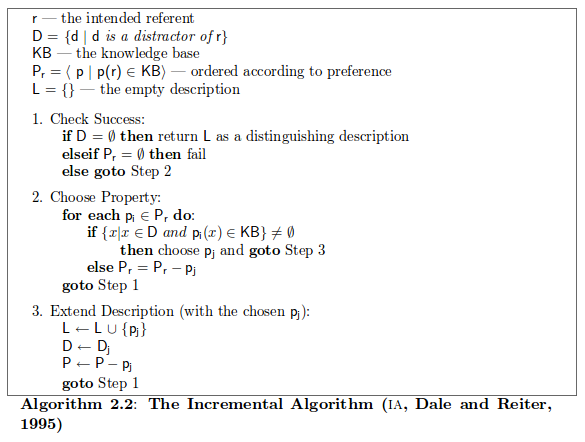
\includegraphics[width=8.5cm]{figures/incremental.png}\\[0pt]
%%\caption{Interface del experimento}
%\label{fig-incremental}
%\end{center}
%\end{figure}


El objeto target que queremos identificar lo llamaremos {\it r},
D es el conjunto de distractores de r,
KB es la base de conocimiento que contiene para cada objeto los valores de sus propiedades.
Tenemos $P_{r}$ propiedad de r que esta inclu\'ida en KB y adem\'as esta ordenado seg\'un preferencia de propiedades.\\
L inicialmente es la descripci\'on vac\'{i}a, al finalizar la ejecusi\'on tendr\'a el conjunto de propiedades con los cuales identificaremos a r.\\

Si D es vaci\'io, no hay nada para identificar, porque no hay distractores.\\

La idea del algoritmo es ir eliminando distractores, por eso, en {\it Paso 1} si no hay distractores, se devuelve L como el conjunto de propiedades que identifica al target. Si todav\'ia hay distractores pero no quedan propiedades de r ($P_{r}$), falla porque no lo puede identificar un\'ivocamente. Si quedan propiedades de r, va al {\it Paso 2}, en el cual elije la propiedad de r que sigue en el orden de preferencias, pero que tambi\'en es propiedad de alg\'un distractor (algun elemento de D) y va al {\it Paso 3}, en caso de que la propiedad no sea propiedad de algun distractor, se actualiza $P_{r}$ a $P_{r}$ menos la propiedad y se va al principio de nuevo.\\
En el {\it Paso 3} se agrega la propiedad a la descripci\'on actual L, se actualiza $D$ con $D_{j}$, es decir con los elementos de $D$ que tienen la propiedad $_j$, se saca $_j$ de la lista de P y continua en {\it Paso 1}.\\

\textcolor{blue}{Un poco mas de historia, no se a donde poner...Theune and Krahmer proposed an extension that allows the generation of subsequent reference with the ia taking into account the discourse salience of the target referent (Krahmer and Theune, 1998; Theune, 2000; Krahmer and Theune, 2002), and a second one which allows the ia to produce referring expressions that
contain binary relations to other objects (Theune, 2000; Krahmer and Theune, 2002). I will return to their relational extension in Section 2.3. Theune and Krahmer's approach works by assigning a salience score to all objects according to the
focus/topic distinction by Hajicova (1993) and Centering Theory (Grosz et al., 1995). They alter the success criterion of the algorithm and only let it stop when here is no distractor left that is as or more salient than the target referent.
Not all properties are the same. The qualitative diferences that exist between diferent properties were first discussed in the
reg literature by van Deemter (2000, 2006). He pointed out that the appropriateness of
vague orgradable properties such as small and large is dependent on the context in which they are used, while,
for example, the colour of an object is absolute. Consider two descriptions in a domain of animals... (van Deemter, 2002), van Deemter considered the ia's logical completeness in terms of the Boolean operators of negation and disjunction. He extended it to
be able to generate referring expressions that contain negated properties, such as Example (2.3), and descriptions of sets of objects, such as Example (2.4), or even (2.5), which contains a logical disjunction of properties. His algorithm proceeds
in stages, trying longer and longer disjunctions of properties, if atomic properties
and shorter disjunctions did not suffice to distinguish the target set.. he work on reference to sets was taken further by Gatt and van Deemter (2005, 2006), who have presented the most mature algorithms in this space to
date. They used a similar procedure to the ia in that their algorithms are based
on incremental processing of a preference order of properties. Their algorithms
add a lot of complex machinery to the basic procedure to ensure that properties
are chosen in a way that maximises coherence within the set of objects described
by the referring expressions. For example, their approach will attempt to use
properties of the same type for all the referents of a set. So, it would produce
descriptions such as Examples (2.6) or (2.7) rather than Example (2.8) or.. }

\subsection{Graph}

Un grafo (del griego grafos:dibujo, imagen) es un conjunto de objetos llamados v\'ertices o nodos unidos por enlaces llamadas aristas o arcos, que permiten representar relaciones binarias entre elementos de un conjunto. \\

Son objeto de estudio de la teor\'{i}a de grafos. \\

Un grafo G es un par ordenado $G=(V,E)$, donde:\\

    V es un conjunto de v\'ertices o nodos, y
    E es un conjunto de aristas o arcos, que relacionan estos nodos.\\

Normalmente V suele ser finito. Muchos resultados importantes sobre grafos no son aplicables para grafos infinitos.\\

Se llama orden del grafo G a su n\'umero de v\'ertices, $|V|$.\\

El grado de un v\'ertice o nodo $v \in V$ es igual al n\'umero de arcos que lo tienen como extremo.\\

Un bucle es una arista que relaciona al mismo nodo; es decir, una arista donde el nodo inicial y el nodo final coinciden.\\

Dos o m\'as aristas son paralelas si relacionan el mismo par de v\'ertices.\\

Un grafo puede ser dirigido o no, etiquetado o no.\\

T\'{i}picamente, un grafo se representa gr\'aficamente como un conjunto de puntos (v\'ertices o nodos) unidos por l\'{i}neas (aristas).\\

Los grafos han sido muy estudiados, pr\'acticamente cualquier problema puede ser expresado como un problema de grafos, y aplicar algoritmos de b\'usqueda ya estudiados.\\

Mirando la obtenci\'on de expresiones referenciales como un problema de grafos, el dominio que incluye al target y los distractores es representado como un grafo dirigido etiquetado. \\

Cada objeto de la escena se modela como un v\'ertice en el grafo. Los atributos at\'omicos como color, tipo o tama\~nno se representan como un bucle en el correspondiente nodo. Est\'an etiquetados con los nombres de las propiedades y los valores que el objeto en cuesti\'on tiene para estas propiedades. \\

Las relaciones binarias entre objetos, por ejemplo abajo-de, arriba-de se modelan como aristas entre los nodos correspondientes.\\

La base de conocimiento que incluye al target ahora esta expresada como los v\'ertices, las aristas y las etiquedas del grafo.\\

%Krahmer et al.'s (2003) reformularon la tarea de seleccionar las propiedades y relaciones que contendr\'a una expresi\'on referencial como un problema de teor\'ia de grafos.

Para generar una descripci\'on distintiva, el algoritmo busca un subgrafo del grafo original que identifica al target un\'{i}vocamente, le llama grafo distintivo (distinguishing graph).\\

Comenzando con el subgrafo que contiene un solo v\'ertice, que representa al target, se realiza una b\'usqueda exaustiva, pero comenzando a lo ancho. \textcolor{blue}{aca hay que escribir mucho mas...} Utiliza una heur\'{i}stica basada en el costo (descripto a continuaci\'on) que es capaz de podar el espacio de b\'usqueda.\\


%esto no se entiende nada
%Informalmente, un subgrafo refiere al target si y s\'olo si puede ser
%`Colocado sobre el gr\'afico de dominio de tal manera que el v\'ertice que representa subgrafo
%del objeto target se puede `coloca sobre 'el v\'ertice del objetivo en el gr\'afico de dominio,
%y cada uno de los bordes marcados en el subgrafo puede ser `coloca sobre 'un correspondiente
%borde en el gr\'afico de dominio con la misma etiqueta y el mismo sentido. Por otra parte,
%un subgrafo distingue al target un\'ivocamente si y s\'olo si se puede `colocarlo sobre grafo original' y es exactamente el
%v\'ertice target. La noci\'on informal de un gr\'afico que se coloca sobre otro corresponde al concepto te\'orico matem\'atico de isomorfismo de grafos.

En teor\'{i}a de grafos, un isomorfismo entre dos grafos G y H es una biyecci\'on f entre los conjuntos de sus v\'ertices $f:V(G) \rightarrow V(H)$ que preserva la relaci\'on de adyacencia. Es decir, cualquier par de v\'ertices u y v de G son adyacentes si y solo si lo son sus im\'agenes, $f(u)$ y $f(v)$, en H.\\

\textcolor{blue}{aca quiero poner un ejemplo que muestre una imagen y el modelo como grafo}

La funci\'on de costo esta definida sobre las aristas y v\'ertices del grafo dominio. El costo de un subgrafo se define como la suma sobre todas las aristas y v\'ertices que contiene el grafo.\\
El algoritmo de b\'usqueda garantiza encontrar el subgrafo de menor costo que representa al target.\\

La funci\'on de costo es usada para podar las ramas del \'arbol de b\'usqueda cuando estas se hacen m\'as costosas que el grafo de menor costo encontrado hasta el momento. Esta funci\'on hace que se prefieran propiedades sobre otras que tienen mayor costo.

\subsection{Bisimulaci\'on}


En este cap\'itulo daremos una introducci\'on a las l\'ogicas de descripci\'on (DL del acr\'onimo en ingl\'es description logic) y luego daremos el algoritmo en el cual nos basamos en esta tesis.\\

La idea es transformar el problema de GER al problema de computar una f\'ormula de DL cuya extensi\'on es el elemento target (o los elementos targets, en el caso de querer dar ER para plurales) aprovechando que una f\'ormula describe un conjunto.\\

Hay distintas l\'ogicas, y entre ellas se diferencian por como se generan, vamos a explicar \alc y \el.\\

\emph{F\'ormulas} (o \emph{conceptos}) $\varphi$ de $\alc$ son generadas por la siguiente gram\'atica:
$$
\varphi,\varphi' ::= \top \mid p \mid \neg \varphi \mid \varphi \sqcap \varphi'
\mid \exists R. \varphi
$$
donde $p$ es el conjunto de los s\'imbolos proposicionales \prop y $R$ es el de los s\'imbolos relacionales \rel. $\el$ es la parte sin negaci\'on de $\alc$.\\

Las f\'ormulas de ambos $\alc$ y $\el$ son interpretadas en modelos relacionales de primer orden $\gM = (\Delta,\interp{\cdot})$ donde
$\Delta$ es un conjunto no vac\'io y $\interp{\cdot}$ es una funci\'on de interpretaci\'on tal que:
$$
\begin{array}{ccl}
\interp{p} & \subseteq & \Delta  \mbox{ para $p \in \prop$}\\
\interp{R} & \subseteq & \Delta \times \Delta  \mbox{ para $R \in \rel$}\\
\interp{\neg \varphi} & = & \Delta - \interp{\varphi}\\
\interp{\varphi \sqcap \varphi'} & = & \interp{\varphi} \cap \interp{\varphi'}\\
\interp{\exists R.\varphi} & = & \{i \mid \mbox{para alg\'un } i', (i,i') \in \interp{R}\\
& & \mbox{ e } i' \in \interp{\varphi} \}.\\
\end{array}
$$

\begin{figure}[ht]
\begin{center}
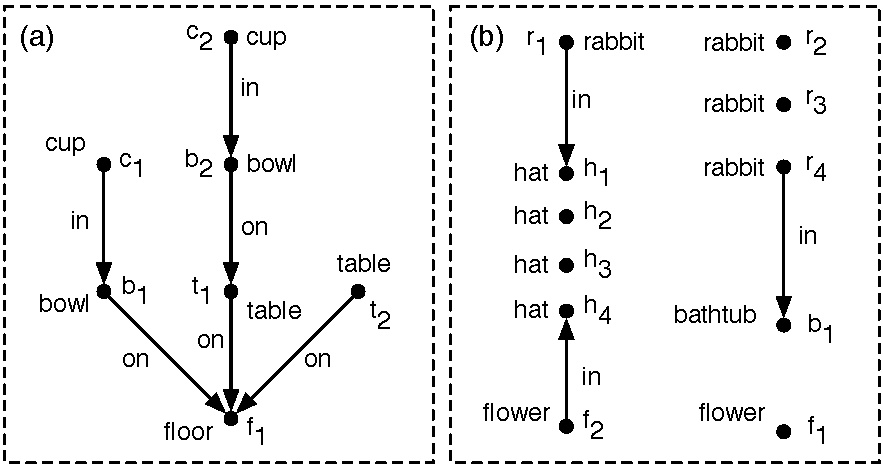
\includegraphics[width=8.5cm]{figures/pic-dale-haddock.pdf}\\[0pt]
\caption{}
\label{fig:dale-haddock}
\end{center}
\end{figure}


Cada f\'ormula de una descripci\'on l\'ogica denota un conjunto de objetos del dominio; por lo tanto podemos usar tales f\'ormulas para describir conjuntos. Por ejemplo en el modelo de la Figura.~\ref{fig:dale-haddock}b, la f\'ormula
$\mathsf{flower}$ denota el conjunto $\{f_1,f_2\}$; La f\'ormula
$\mathsf{flower} \sqcap \exists \mathsf{in}.\mathsf{hat}$ denota
$\{f_2\}$; y la f\'ormula $\mathsf{flower} \sqcap \neg
\exists \mathsf{in}.\mathsf{hat}$ denota $\{f_1\}$.\\

\textcolor{blue}{no se si dejar este ejemplo, o cambiarlo por uno es espa\~nol}

Hay muchas otras l\'ogicas de descripci\'on (DL) en la literatura por ejemplo 

$\mathcal{CL}$ (\el\ sin el cuantificador existencial, es decir solo conjunciones at\'omicas); $\mathcal{PL}$ (\alc\ l\'ogica propocisional); y
$\mathcal{ELU}_{(\neg)}$ (\el\ m\'as disjunci\'on y negaci\'on at\'omica).\\

Usaremos una noci\'on de preservaci\'on de f\'ormulas que llamaremos
\emph{similaridad}. Para cualquier DL $\gL$, diremos que un individual $i$ es \emph{\gL-similar} a $i'$ en un modelo dado $\gM$
si para cualquier f\'ormula $\varphi \in \gL$ tal que $i \in
\interp{\varphi}$, tambi\'en tenemos que $i' \in \interp{\varphi}$.\\
Equivalentemente, no hay $\gL$-f\'ormula que se mantenga para $i$ pero no para
$i'$.  Diremos que el \emph{\gL-conjunto de similaridad} de alg\'un individual
$i$ es el conjunto de todos los individuales a los cuales $i$ es \gL-similar.\\

Notar que la similaridad no es necesariamente una relaci\'on sim\'etrica: Por ejemplo:$f_1$ es \el-similar a $f_2$ en
Figura~\ref{fig:dale-haddock}b, pero $f_2$ no es \el-similar a $f_1$
(satisface la f\'ormula $\exists \mathsf{in}.\mathsf{hat}$ y $f_1$
no la satisface).  De todas maneras, \alc-similaridad es una relaci\'on sim\'etrica porque
el languaje contiene negaci\'on; y en consecuencia, $f_1$ no es \alc-similar
a $f_2$ porque este tampoco satisface $\neg \exists
\mathsf{in}.\mathsf{hat}$.  Porque \alc\ es m\'as expresivo que \el,
esto es, para alg\'un individual $a$ es posible ser \el-similar pero
no \alc-similar a alg\'un individual $b$, pero no viceversa.\\



\textcolor{blue}{SACAR ESTO... poner quizas en la introduccion o en primer capitulo. Las ER que involucran relaciones han recibido m\'as atenci\'on recientemente;
especialmente en el contexto de las expresiones referenciales espaciales en 
generaci\'on (por ejemplo,~\cite{kelleher06:increm}),
donde es particularmente natural utilizar expresiones que implican 
relaciones espaciales, tales como ``la pelota en la parte superior del cubo''. Sin embargo, el
algoritmo cl\'asico
por~\cite{dale91:gener} ha demostrado ser
incapaz de generar ER satisfactorias en la pr\'actica (v\'ease el an\'alisis sobre
el~\emph{cabinet corpus}
en~\cite{viethen06:_algor_for_gener_refer_expres}). Adem\'as, el
Dale y Haddock algoritmo y muchos de sus sucesores (tales
como~\cite{kelleher06:increm}) son vulnerables a
el problema de la \emph{regresi\'on infinita}, donde el algoritmo entra en un
bucle infinito, saltando hacia atr\'as y hacia adelante entre las descripciones para dos
individuos emparentados, como en `` el libro sobre la mesa que soporta una
libro sobre la mesa \ldots ''}

%REs involving relations have received increasing attention recently;
%especially in the context of spatial referring expressions in situated
%generation (e.g., \cite{kelleher06:increm}),
%where it is particularly natural to use expressions involving spatial
%relations such as ``the ball on top of the cube.''  However, the
%classical algorithm
%by~\cite{dale91:gener} was shown to be
%unable to generate satisfying REs in practice (see the analysis over
%the \emph{cabinet corpus}
%in~\cite{viethen06:_algor_for_gener_refer_expres}).  Furthermore, the
%Dale and Haddock algorithm and many of its successors (such
%as~\cite{kelleher06:increm}) are vulnerable to
%the problem of \emph{infinite regress}, where the algorithm enters an
%infinite loop, jumping back and forth between descriptions for two
%related individuals, as in ``the book on the table which supports a
%book on the table \ldots''

%\cite{arec2:2008:Areces,arec:usin11} have proposed low complexity
%algorithms for the generation of relational REs
%%(including references to sets) 
%that eliminate the risk of infinite regression.  These algorithms are
%based on variations of the partition refinement algorithms
%of~\cite{paig:thre87}.  The information provided by a given scene
%is interpreted as a relational model whose objects are classified into
%sets that fit the same description.  This classification is
%successively \emph{refined} till the target is the only element
%fitting the description of its class.  The existence of an ER depends
%on the information available in the input scene, and on the expressive
%power of the formal language used to describe elements of the
%different classes in the refinement.


\cite{arec2:2008:Areces,arec:usin11} han propuesto algoritmos de baja complejidad
 para la generaci\'on de ER relacionales que eliminan el riesgo de regresi\'on infinita. Estos algoritmos son
basado en variaciones de los algoritmos de refinamiento particiones
de~\cite{paig:thre87}. La informaci\'on proporcionada por una escena dada
se interpreta como un modelo relacional cuyos objetos se clasifican en
conjuntos que se adaptan a la misma descripci\'on. Esta clasificaci\'on es
conjuntos que se adaptan a la misma descripci\'on. Esta clasificaci\'on es
sucesivamente \emph{refinada} hasta que el target es el \'unico elemento
en la clase. La existencia de un ER depende
de la informaci\'on disponible en la escena de entrada, y en el poder expresivo
del lenguaje formal utilizado para describir los elementos de las
diferentes clases en el refinamiento.\\

%Refinement
%algorithms %presented in~\cite{arec2:2008:Areces,arec:usin11}
%effectively compute REs for all individuals in the domain, at the same
%time. The algorithms always terminate returning a formula of the
%formal language chosen that uniquely describes the target (if the
%formal language is expressive enough to identify the target in the
%input model).
%\cite{arec2:2008:Areces}
%show that the refinement algorithm using the description language \el  is capable of generating 67\% of 
%the relational REs in the~\cite{viethen06:_algor_for_gener_refer_expres} dataset, when all possible orders of the relations in the domain are considered. This is in sharp contrast with the analysis 
%done in~\cite{viethen06:_algor_for_gener_refer_expres} over the cabinet corpus, of algorithms based in Dale and Reiter's original proposal.    

Los algoritmos de refinamiento
% presenta en~\cite{arec 2:2008:Areces, arec:usin11}
calculan efectivamente ER para todos los objetos en el dominio, al mismo
tiempo. Los algoritmos siempre terminan devolviendo una f\'ormula del
lenguaje formal elegido que describe un\'{i}vocamente el objetivo (si el
lenguaje formal es suficientemente expresivo para identificar el target en el
modelo de entrada).\\

%Refinement algorithms for GER are based on the following basic idea:
%given a scene $S$, the objects appearing in $S$ are successively
%classified according to their properties into finer and finer
%classes. A description (in some formal language $\mathcal{L}$) of each
%class is computed every time a class is refined. The procedure always
%stops when the set of classes stabilizes, i.e., no further refinement
%is possible with the information available in the scene\footnote{Of
%  course, if we are only interested in a referring expression for a
%  given target we can stop the procedure as soon as the target is the
%  only element of some of the classes.}.  If the target element is in
%a singleton class, then the formal description of that class is a
%referring expression; otherwise the target cannot be unequivocally
%described (in 

Algoritmos de refinamiento para GER se basan en la siguiente idea b\'asica:
dada una escena $S$, los objetos que aparecen en $S$ son sucesivamente
clasificados de acuerdo con sus propiedades en clases m\'as y m\'as finas. 
Una descripci\'on (en alg\'un lenguaje formal de $\mathcal{L}$) de cada
clase se calcula cada vez que una clase es refinada. El procedimiento siempre
se detiene cuando el conjunto de clases se estabiliza, es decir, no se puede hacer m\'as refinamiento
con la informaci\'on disponible en la escena \footnote{Por supuesto, si s\'olo estamos interesados en una expresi\'on referencial de un objeto dado, se puede detener el procedimiento en cuanto el objetivo es el
   \'unico elemento de alguna de las clases.}. Si el elemento target est\'a en
una clase singleton, entonces la descripci\'on formal de esa clase es un
expresi\'on referencial; de lo contrario el target no puede ser un\'{i}vocamente
descripto (en $\mathcal{L}$).\\

%It is clear that a scene can be encoded in different ways as a
%relational model (for example in \ref{figure22}, we could argue that
%$e_1$ is also \emph{leftof} $e_2$, not considered because they are no
%touching). The algorithm assumes that these issues have been resolved
%and that the model encodes a suitable representation of the scene we
%want to describe.  Moreover, we will assume that all relations are
%\emph{binary}.  We will not consider relations of arity greater than
%two (relations of higher arity can be encoded as binary relations via
%reification, if necessary).

\begin{figure}[ht]
\begin{minipage}[b]{0.45\linewidth}
\centering
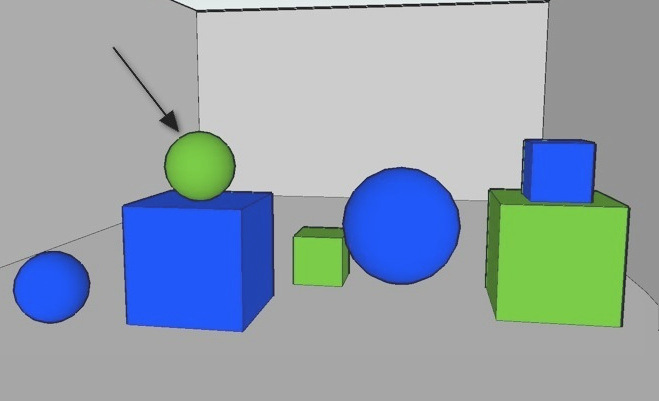
\includegraphics[width=\textwidth]{images/3.jpg}
\vspace*{1cm}
%\caption{Input scene}
\label{GRE3D7-stimulus}
\end{minipage}
%\hspace*{-0.35cm}
\begin{minipage}[b]{0.6\linewidth}
\centering
\begin{tikzpicture}
  [
    n/.style={circle,fill,draw,inner sep=3pt,node distance=1.4cm},
    aArrow/.style={->, >=stealth, semithick, shorten <= 2pt, shorten >= 2pt},
  ]
 \node[n,label=above:$e_1$,label=below:{
    \relsize{-1}$\begin{array}{c}
      \nLeft\\[-2pt]
      \nSmall\\[-2pt] 
      \nBlue \\[-2pt] 
      \nBall\end{array}$}] (a) {};

 \node[n,label=above:$e_2$,label=below:{
    \relsize{-1}$\begin{array}{c}
      \nLeft\\[-2pt]
      \nBig\\[-2pt] 
      \nBlue\\[-2pt] 
      \nCube\end{array}$}, right of=a] (b) {};

 \node[n,label=below:$e_3$,label=above:{
    \relsize{-1}$\begin{array}{c}
      \nTop\\[-2pt]
      \nLeft\\[-2pt]
      \nSmall\\[-2pt] 
      \nGreen\\[-2pt] 
      \nBall\end{array}$}, above of=b] (c) {};

 \node[n,label=above:$e_4$,label=below:{
    \relsize{-1}$\begin{array}{c}
      \nSmall\\[-2pt] 
      \nGreen\\[-2pt] 
      \nCube\end{array}$}, right of=b] (d) {};

 \node[n,label=above:$e_5$,label=below:{
    \relsize{-1}$\begin{array}{c}
      \nBig\\[-2pt] 
      \nBlue\\[-2pt] 
      \nBall\end{array}$}, right of=d] (e) {};

 \node[n,label=above:$e_6$,label=below:{
    \relsize{-1}$\begin{array}{c}
      \nBig\\[-2pt] 
      \nGreen\\[-2pt] 
      \nCube\end{array}$}, right of=e] (f) {};

 \node[n,label=below:$e_7$,label=above:{
    \relsize{-1}$\begin{array}{c}
      \nTop\\[-2pt]
      \nSmall\\[-2pt] 
      \nBlue\\[-2pt] 
      \nCube\end{array}$}, above of=f] (g) {};

 \draw [aArrow,bend right=90] (b) to node[auto,swap]{\relsize{-1}$\nBelow$} (c);
 \draw [aArrow,bend right=90] (c) to node[auto,swap]{\relsize{-1}$\nOntop$} (b);

 \draw [aArrow,bend right=30] (d) to node[auto,swap]{\relsize{-1}$\nLeftof$} (e);
 \draw [aArrow,bend right=30] (e) to node[auto,swap]{\relsize{-1}$\nRightof$} (d);

 \draw [aArrow,bend right=90] (f) to node[auto,swap]{\relsize{-1}$\nBelow$} (g);
 \draw [aArrow,bend right=90] (g) to node[auto,swap]{\relsize{-1}$\nOntop$} (f);

 \draw[dotted] (-.5,-1.4) rectangle (7.1,3.1);

 \end{tikzpicture}
\caption{Escena como un modelo relacional}
\label{GRE3D7-stimulus-graph}
\end{minipage}
\end{figure}

Est\'a claro que una escena puede ser codificada en diferentes formas como un
modelo relacional (por ejemplo, en \ref{GRE3D7-stimulus}, podr\'{i}amos argumentar que
$e_1$ es tambi\'en \emph{leftof} $e_2$, pero no lo consideramos porque no se estan 
tocando). El algoritmo asume que estas cuestiones se han resuelto y que el modelo codifica una representaci\'on adecuada de la escena que
queremos describir. Por otra parte, vamos a suponer que todas las relaciones son
\emph{binarias}. No vamos a considerar las relaciones de aridad mayor que
dos (relaciones de mayor aridad pueden codificarse como relaciones binarias v\'{i}a
reificaci\'on, si es necesario).\\

%On termination, the algorithm computes what are called the
%$\mathcal{L}$-similarity classes of the input model $\gM$.
%Intuitively, the referring expression ``\textsf{ball}'' and ``\textsf{cube}''  are more specific and then contain more information than $\top$.


Tras la resoluci\'on, el algoritmo calcula lo que se llama la
$\mathcal{L}$ - clases de semejanza del modelo de entrada de $\gM$.\\

%There is many $\mathcal{L}$, we will name $\alc$ and $\el$

%ACA VOY A PONER gramatica para generar... ALC y EL no quedaria bien aca, hay que ver lo agregamos antes o no hace falta
%In what follows, we use formulas of the $\el$ description logic
%language
En lo que sigue, se utilizan f\'ormulas de la descripci\'on de la l\'ogica $\el$
~\cite{baad:desc03} para describir las clases de refinamiendo
\footnote{N\'otese, sin embargo, que el lenguaje formal particular usado es
   independiente del algoritmo principal, y diferentes funciones
  add$_{\mathcal{L}}$($\varphi$,\RE) se pueden utilizar dependiendo
   de la l\'ogica en cuesti\'on.}. como se discuti\'o 
en~\cite{arec2:2008:Areces}, 
este lenguaje es adecuado para describir
RE conjuntivas y relacionales, que son lo que encontramos en los corpus.

  La entrada al algoritmo ser\'a un modelo $\mathcal{M} =
 \tup{\Delta, \interp{\cdot}}$, donde $\Delta$ es el dominio no vac\'io de objetos de la imagen,
 $\interp{\cdot}$ es una funci\'on de interpretaci\'on que asigna a todas las propiedades de la escena su extensi\'on.
 Por ejemplo, la escena mostrada en la Figura~\ref{GRE3D7-stimulus} podr\'ia ser representada por el modelo
 $\gM=\tup{\Delta,\interp{\cdot}}$ mostrado en la 
 Figura~\ref{GRE3D7-stimulus-graph}; donde+- $\Delta =
 \{e_1,\ldots,e_7\}$, e $\interp{\textsf{red}}$ is $\{e_2, e_4, e_5,
 e_7\}$.

$\top$ es una f\'ormula que representa la descripci\'on m\'as general, cuya
interpretaci\'on incluye todos los elementos del modelo. Se podr\'ia realizar
como la ER con el sustantivo
``\textsf{cosa}''. Decimos que una f\'ormula es
\emph{subsumed} por otras f\'ormulas, la su extensi\'on puede ser cubierta por la
union de las extensiones de las otras f\'ormulas. Por ejemplo, en la
Figura~\ref{GRE3D7-stimulus}, $\top$ es subsumida por ``\textsf{ball}'' y
``\textsf{cube}'', porque $\interp{\top}$ = $\interp{\textsf{ball}}
\cup \interp{\textsf{cube}}$.
%= $\{e_2, e_4, e_6, e_7\}$, it is $\{e_1, e_2, e_3, e_4, e_5, e_6, e_7\}$ = $\{e_1, e_3, e_5\} \cup \{e_2, e_4, e_6, e_7\}$. 
Intuitivamente la f\'ormula ``\textsf{cube}'' o ``\textsf{ball}'' tienen m\'as informaci\'on que $\top$, para cada elemento de $\top$, hay una f\'ormula que d\'a m\'as informaci\'on, digamos ``\textsf{cube}'' es m\'as informativa que ``\textsf{thing}''.\\

%In the following we will explain an example of execusion of the
%algorithm shown in Figure
A continuaci\'on vamos a explicar un ejemplo de ejecusi\'on del
algoritmo mostrado en la Figura~\ref{algoritmoOriginal} considerando la l\'ogica 
$\el$ como language. Este algoritmo fue presentado en
~\cite{arec2:2008:Areces}.

\begin{figure}[h!]
\begin{center}
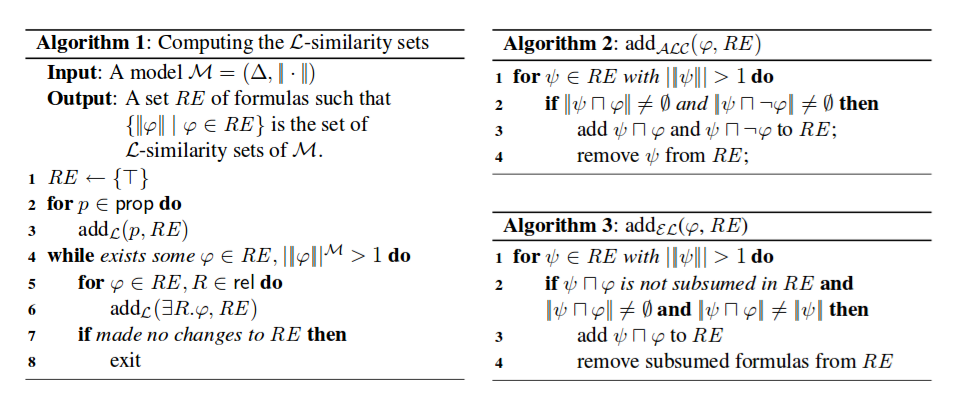
\includegraphics[width=\textwidth]{images/algoritmoOriginal.png}
\end{center}
\vspace*{-2em}
\caption{Algoritmo para GER con l\'ogicas de descripci\'on}
\label{algoritmoOriginal}
\end{figure}

\subsection{Ejemplo de ejecuci\'on}

\textcolor{blue}{no se si poner aca un ejemplo, si poner el texto y las im\'agenes en otro apendice... o ponerlas mas chiquitas en varias columnas, asi queda feo}
Vamos a ejecutar el algoritmo para la Figura~\ref{GRE3D7-stimulus},
el algoritmo comienza con una lista fija de propiedades y relaciones, supongamos que
esas listas son las siguientes:

propiedades ordenadas (prop): \textsf{ball}, \textsf{cube}, \textsf{red}, \textsf{yellow}, \textsf{small}, \textsf{large}.\\
relaciones ordenadas (rel): \textsf{leftof}, \textsf{rightof}, \textsf{ontopof}, \textsf{bellowof}.

%\begin{figure}
%\begin{center}	
%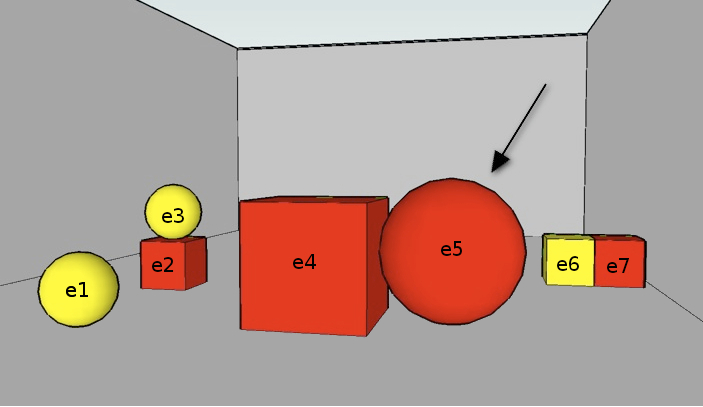
\includegraphics[width=.5\textwidth]{images/22.jpg}
%\end{center}
%\vspace*{-1.5em}
%\caption{Escena 3D de figuras geom\'etricas}\label{figure22}
%\end{figure}

%\begin{figure}
%\begin{minipage}[b]{0.6\linewidth}
%\centering
%\begin{tikzpicture}
%  [
%    n/.style={circle,fill,draw,inner sep=3pt,node distance=1.4cm},
%    aArrow/.style={->, >=stealth, semithick, shorten <= 2pt, shorten >= 2pt},
%  ]
% \node[n,label=above:$e_1$,label=below:{
%    \relsize{-1}$\begin{array}{c}
%      \nLeft\\[-2pt]
%      \nSmall\\[-2pt] 
%      \nYellow \\[-2pt] 
%      \nBall\end{array}$}] (a) {};

% \node[n,label=above:$e_2$,label=below:{
%    \relsize{-1}$\begin{array}{c}
%      \nLeft\\[-2pt]
%      \nSmall\\[-2pt] 
%      \nRed\\[-2pt] 
%      \nCube\end{array}$}, right of=a] (b) {};

% \node[n,label=below:$e_3$,label=above:{
%    \relsize{-1}$\begin{array}{c}
%      \nTop\\[-2pt]
%      \nLeft\\[-2pt]
%      \nSmall\\[-2pt] 
%      \nYellow\\[-2pt] 
%      \nBall\end{array}$}, above of=b] (c) {};

% \node[n,label=above:$e_4$,label=below:{
%    \relsize{-1}$\begin{array}{c}
%      \nBig\\[-2pt] 
%      \nRed\\[-2pt] 
%      \nCube\end{array}$}, right of=b] (d) {};

% \node[n,label=above:$e_5$,label=below:{
%    \relsize{-1}$\begin{array}{c}
%      \nBig\\[-2pt] 
%      \nRed\\[-2pt] 
%      \nBall\end{array}$}, right of=d] (e) {};

% \node[n,label=above:$e_6$,label=below:{
%    \relsize{-1}$\begin{array}{c}
%      \nSmall\\[-2pt] 
%      \nYellow\\[-2pt] 
%      \nCube\end{array}$}, right of=e] (f) {};

% \node[n,label=above:$e_7$,label=below:{
%    \relsize{-1}$\begin{array}{c}
%      \nSmall\\[-2pt] 
%      \nRed\\[-2pt] 
%      \nCube\end{array}$}, right of=f] (g) {};

% \draw [aArrow,bend right=90] (b) to node[auto,swap]{\relsize{-1}$\nBelow$} (c);
% \draw [aArrow,bend right=90] (c) to node[auto,swap]{\relsize{-1}$\nOntop$} (b);

% \draw [aArrow,bend right=30] (d) to node[auto,swap]{\relsize{-1}$\nLeftof$} (e);
% \draw [aArrow,bend right=30] (e) to node[auto,swap]{\relsize{-1}$\nRightof$} (d);

% \draw [aArrow,bend right=30] (f) to node[auto,swap]{\relsize{-1}$\nLeftof$} (g);
% \draw [aArrow,bend right=30] (g) to node[auto,swap]{\relsize{-1}$\nRightof$} (f);

% \draw[dotted] (-.4,-1.7) rectangle (7.5,3.3);

% \end{tikzpicture}
%\caption{La escena como modelo relacional}\label{GRE3D7-stimulus-graph}
%\end{minipage}
%\end{figure}


El algoritmo siempre termina, y devuelve ER un conjunto de f\'ormulas que describe cada elemento en el dominio (si existe esa f\'ormula). \\

En el comienzo ER=$\{\top\}$ y $\interp{\top}$ = $\{e_1, e_2, e_3, e_4, e_5, e_6, e_7\}$ como se puede ver en la Figura~\ref{fig-modelo}.\\

\begin{figure}[ht]
\begin{center}
\frame{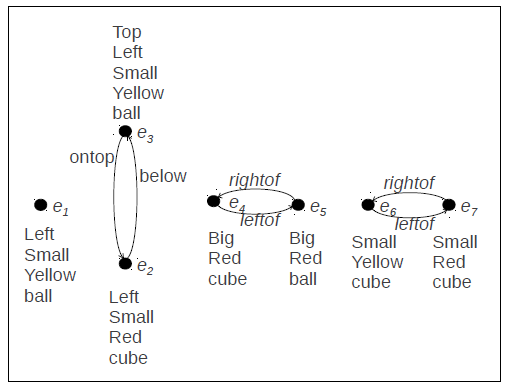
\includegraphics[width=8cm]{images/modelo.png}}\\[0pt]
\caption{Modelo de la Figura \ref{GRE3D7-stimulus}}
\label{fig-modelo}
\end{center}
\end{figure}
El primer bucle del algoritmo es en las propiedades. Para cada propiedad hace add$_\el$ ($\varphi$, RE), las propiedades at\'omicas se muestran en la Figura~\ref{fig-modelo2}.

\begin{figure}[ht]
\begin{center}
\frame{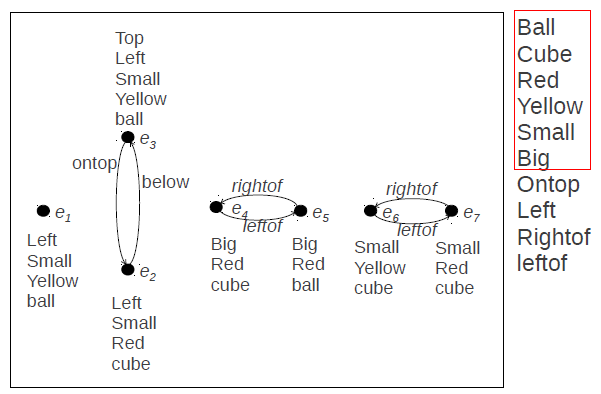
\includegraphics[width=8cm]{images/modelo2.png}}\\[0pt]
\caption{Propiedades proposicionales en cuadro rojo, las del primer ciclo del algoritmo}
\label{fig-modelo2}
\end{center}
\end{figure}

La f\'ormula $\varphi$ se a\~nadir\'a a ER si su interpretaci\'on tiene al menos un elemento, a continuaci\'on, para cada f\'ormula
 $\psi$ en ER la conjunci\'on
$\varphi  \wedge \psi$ no necesita estar subsumida in ER, la $\interp{\varphi \cup \psi}$ no tiene que ser vac\'io, y su interpretaci\'on tiene que ser distinta de $\interp{\psi}$. Luego las f\'ormulas subsumidas se borran.

La primer propiedad es \textsf{ball}, ER = \{$\top$, \textsf{ball}\}, se ven los elementos de ``ball'' en un recuadro en la Figura~\ref{fig-modelo3}.

\begin{figure}[ht]
\begin{center}
\frame{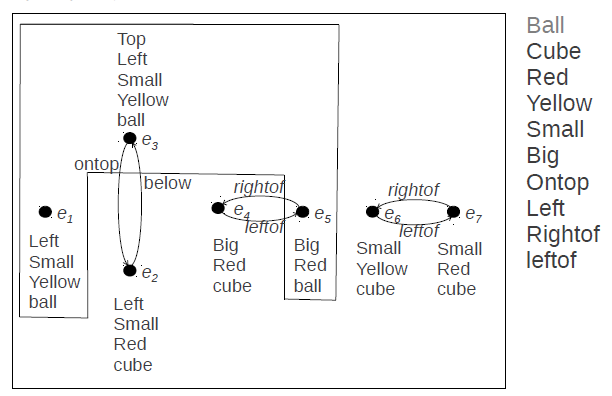
\includegraphics[width=8cm]{images/modelo3.png}}\\[0pt]
\caption{El cuadro indica cuales son ``ball''}
\label{fig-modelo3}
\end{center}
\end{figure}

La siguiente propiedad es \textsf{cube}, ER = \{$\top$, \textsf{ball}, \textsf{cube}\}, pero ahora la $\interp{\textsf{ball}}$ = $\{e_1, e_3, e_5\}$, $\interp{\textsf{cube}}$ = $\{e_2, e_4, e_6, e_7\}$, quedando las particiones como se muestra en la Figura~\ref{fig-modelo4}
\begin{figure}[ht]
\begin{center}
\frame{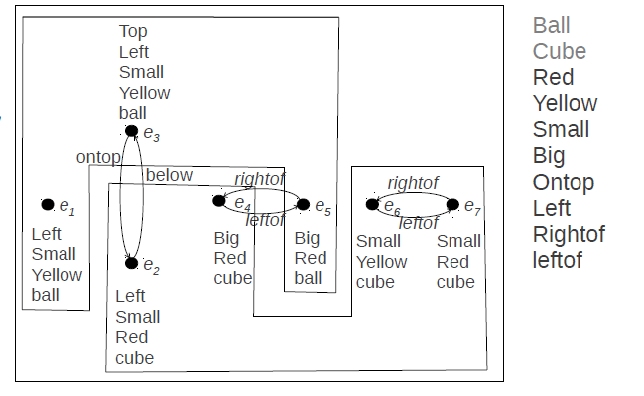
\includegraphics[width=8cm]{images/modelo4.png}}\\[0pt]
\caption{Cuadros indicando ``ball'' y ``cube''}
\label{fig-modelo4}
\end{center}
\end{figure}
Ahora podemos borrar $\top$, porque es subsumida (esta cubierta por) a las otras dos f\'ormulas. La siguiente propiedad es  \textsf{red}, $\interp{\textsf{red}}$ es: $\{e_2, e_4, e_5, e_7\}$, haciendo la intersecci\'on con la $\interp{.}$ de cada f\'ormula en ER obtenemos, $\{e_5\}$ y $\{e_2, e_4, e_7\}$, ER = $\{\textsf{ball}, \textsf{cube}, \textsf{ball} \wedge \textsf{red}, \textsf{cube} \wedge \textsf{red}\}$, las particiones actuales se pueden ver en la Figura~\ref{fig-modelo9}.
\begin{figure}[ht]
\begin{center}
\frame{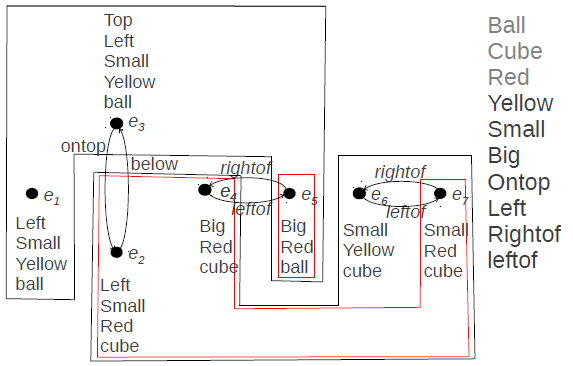
\includegraphics[width=8cm]{images/modelo9.png}}\\[0pt]
\caption{Cuadros indicando ``ball'', ``cube'' y ``red''}
\label{fig-modelo9}
\end{center}
\end{figure}

Siguiendo con \textsf{yellow}, tenemos, $\interp{\textsf{yellow}}$ = $\{e_1, e_3, e_6\}$ y obtenemos ER = $\{\textsf{ball} \wedge \textsf{yellow}, \textsf{cube} \wedge \textsf{yellow}, \textsf{ball} \wedge \textsf{red}, \textsf{cube} \wedge \textsf{red}\}$. 
Note que aqu\'i ya borramos la f\'ormula \textsf{ball} porque estaba subsumida, y la f\'ormula \textsf{cube} tambi\'en. Se muestran particiones en Figura~\ref{fig-modelo10}.

\begin{figure}[ht]
\begin{center}
\frame{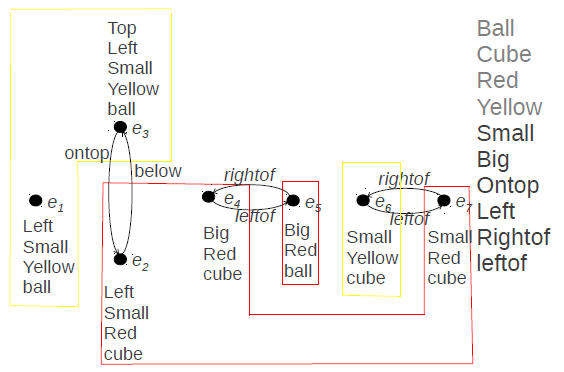
\includegraphics[width=8cm]{images/modelo10.png}}\\[0pt]
\caption{Cuadros indicando ``ball'', ``cube'', ``red'' y ``yellow''}
\label{fig-modelo10}
\end{center}
\end{figure}

Haciendo lo mismo con \textsf{small} tenemos ER = $\{\textsf{ball} \wedge \textsf{yellow} \wedge \textsf{small}, \textsf{cube} \wedge \textsf{yellow} \wedge \textsf{small}, \textsf{ball} \wedge \textsf{red}, \textsf{cube} \wedge \textsf{red}, \textsf{cube} \wedge \textsf{red} \wedge \textsf{small}\}$, como se puede ver en Figura~\ref{fig-modelo11}.
\begin{figure}[ht]
\begin{center}
\frame{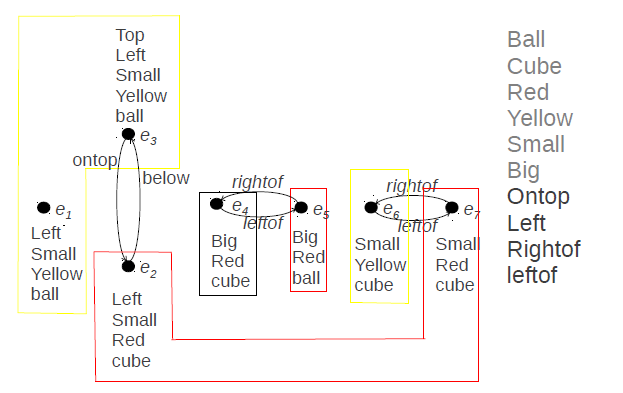
\includegraphics[width=8cm]{images/modelo11.png}}\\[0pt]
\caption{Cuadros indicando ``ball'', ``cube'', ``red'', ``yellow'', ``small'' y ``large''}
\label{fig-modelo11}
\end{center}
\end{figure}

La siguiente propiedad es \textsf{large} as\'i, tenemos ER = $\{\textsf{ball} \wedge \textsf{yellow} \wedge \textsf{small}, \textsf{cube} \wedge \textsf{yellow} \wedge \textsf{small}, \textsf{ball} \wedge \textsf{red}, \textsf{cube} \wedge \textsf{red} \wedge \textsf{large}, \textsf{cube} \wedge \textsf{red} \wedge \textsf{small}\}$. Aqu\'i no podemos agregar \textsf{large} a la f\'ormula $\textsf{red} \wedge \textsf{cube}$ porque su interpretaci\'on tiene un solo elemento, y la condici\'on dice que es necesario tener m\'as de uno.

Hasta ahora ER = $\{\textsf{ball} \wedge \textsf{yellow} \wedge \textsf{small}, \textsf{cube} \wedge \textsf{yellow} \wedge \textsf{small}, \textsf{ball} \wedge \textsf{red}, \textsf{cube} \wedge \textsf{red} \wedge \textsf{large}, \textsf{cube} \wedge \textsf{red} \wedge \textsf{small}\}$ 
y tenemos las siguientes extensiones: $\{e_1, e_3\}, \{e_6\}, \{e_5\}, \{e_4\}, \{e_2, e_7\}$ respectivamente. 
Hay dos f\'ormulas que a\'un pueden ser refinadas, $\textsf{ball} \wedge \textsf{yellow} \wedge \textsf{small}$ y $\textsf{cube} \wedge \textsf{red} \wedge \textsf{small}$ 
debido a que tienen m\'as de un elemento cada una, por lo que entran en el ciclo, while del algoritmo 1, en la l\'inea 4. Ahora es el turno de las relaciones, la primera de ellas es \textsf{leftof}, para cada f\'ormula $\varphi$ en ER trataremos de hacer add$_\el$ ($\exists \textsf{leftof}.\varphi$, RE). Notar que $\psi$ solo puede ser $\textsf{ball} \wedge \textsf{yellow} \wedge \textsf{small}$ o $\textsf{cube} \wedge \textsf{red} \wedge \textsf{small}$ porque esos son los que su interpretaci\'on tiene m\'as de un elemento. 
\begin{figure}[ht]
\begin{center}
\frame{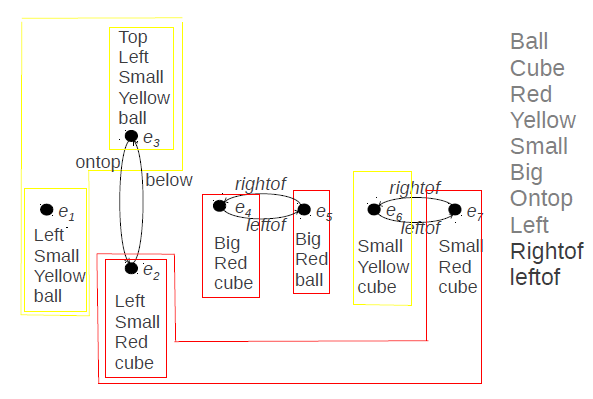
\includegraphics[width=8cm]{images/modelo15.png}}\\[0pt]
\caption{Cuadros indicando ``ball'', ``cube'', ``red'', ``yellow''...}
\label{fig-modelo15}
\end{center}
\end{figure}


No hay
%because those are the ones that its interpretation have more than one element. There is not 
$\varphi$ y $\psi$ que puedan ser aplicadas. Continuando con \textsf{rightof} agregamos $\textsf{cube} \wedge \textsf{yellow} \wedge \textsf{small} \wedge \exists \textsf{rightof}. \textsf{cube} \wedge \textsf{red} \wedge \textsf{small}$, y asi con \textsf{topof} agregamos $\textsf{small} \wedge \textsf{red} \wedge \textsf{cube} \wedge \exists \textsf{ontop}. \textsf{small} \wedge \textsf{yellow} \wedge \textsf{ball}$ y el algoritmo termina con ER = $\{\textsf{ball} \wedge \textsf{yellow} \wedge \textsf{small}, \textsf{cube} \wedge \textsf{yellow} \wedge \textsf{small}, \textsf{ball} \wedge \textsf{red}, \textsf{cube} \wedge \textsf{red} \wedge \textsf{large}, \textsf{cube} \wedge \textsf{red} \wedge \textsf{small}, \textsf{cube} \wedge \textsf{yellow} \wedge \textsf{small} \wedge \exists \textsf{rightof}. \textsf{cube} \wedge \textsf{red} \wedge \textsf{small}, \textsf{small} \wedge \textsf{red} \wedge \textsf{cube} \wedge \exists \textsf{ontop}. \textsf{small} \wedge \textsf{yellow} \wedge \textsf{ball}\}$, 
aqu\'i todos los elementos est\'an en una clase singleton y no se puede hacer ning\'un refinamiento m\'as. 
%can be applied to $cube \wedge red \wedge small$ but there is no formula which interpretation has more than one element to be apply with this one. The same happen for the other relations, so the algorithm ends.
%its interpretation is $\{e_7\}$ with $\psi$ is $cube \wedge yellow \wedge small$, the others combinations can't be apply because they don't do true the preconditions. The following relation is rightof, 

%leftof, rightof, ontopof, bellowof

%At this point we already have the target in a singleton set. So the formula for it is ``red and ball'', and also for s6 which formula is ``yellow cube''.\\
%As we show this algorithm depends of the order of properties and relations.\\
\begin{figure}[ht]
\begin{center}
\frame{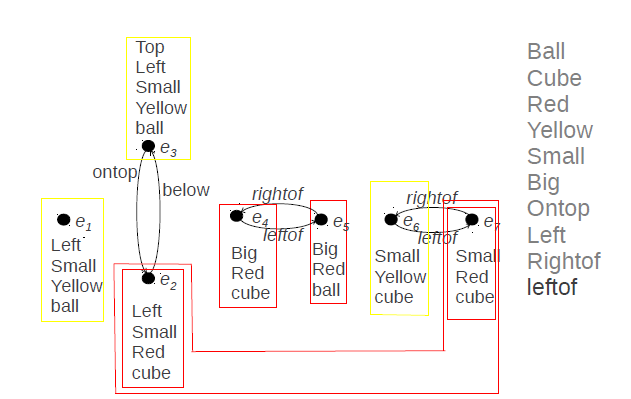
\includegraphics[width=8cm]{images/modelo16.png}}\\[0pt]
\caption{Cuadros indicando ``ball'', ``cube'', ``red'', ``yellow''...}
\label{fig-modelo16}
\end{center}
\end{figure}

\begin{figure}[ht]
\begin{center}
\frame{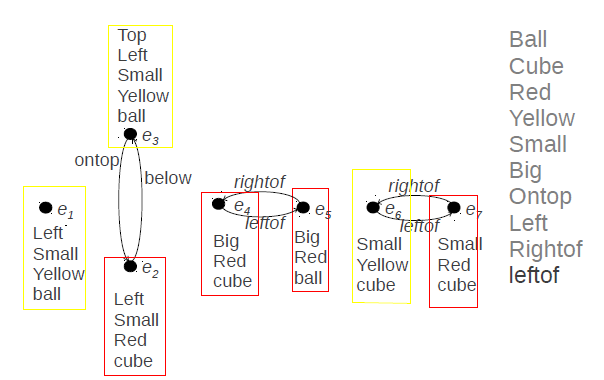
\includegraphics[width=8cm]{images/modelo17.png}}\\[0pt]
\caption{Cuadros indicando ``ball'', ``cube'', ``red'', ``yellow''...}
\label{fig-modelo17}
\end{center}
\end{figure}

\section{Aproximaciones emp\'iricas a la soluci\'on de REG}

\subsection{Corpus existente}

\label{sec:corpusTUNA}

%was the first prominent REG corpus to be made publicly available for research purposes. The corpus was developed in a series of general-purpose controlled experiments, containing 2280 descriptions produced by 60 speakers in two domains (1200 descriptions of furniture items and 1080 descriptions of people's photographs). TUNA does not contain relational descriptions, and it is possibly the only resource of this kind to include situations of reference to sets. The TUNA corpus has been extensively used in a series of shared tasks

TUNA \cite{tuna-corpus} fue el primer corpus prominente para GER disponible p\'ublicamente con fines de investigaci\'on. El corpus fue desarrollado en una serie de experimentos controlados de prop\'osito general, contiene 2.280 descripciones producidas por 60 personas en dos dominios (1.200 expresiones referenciales de im\'agenes de muebles y 1080 expresiones referenciales de fotograf\'ias de personas situadas en una imagen). TUNA no contiene descripciones relacionales, y es posiblemente el \'unico recurso de este tipo para incluir situaciones de referencia a conjuntos. El corpus TUNA se ha utilizado ampliamente en una serie de desaf\'ios \cite{reg2009}. Se muestran ejemplos de im\'agenes en Figuras \ref{fig-TUNA-furniture} y \ref{fig-TUNA-people}

\begin{figure}
\begin{minipage}[t]{0.5\linewidth}
\centering
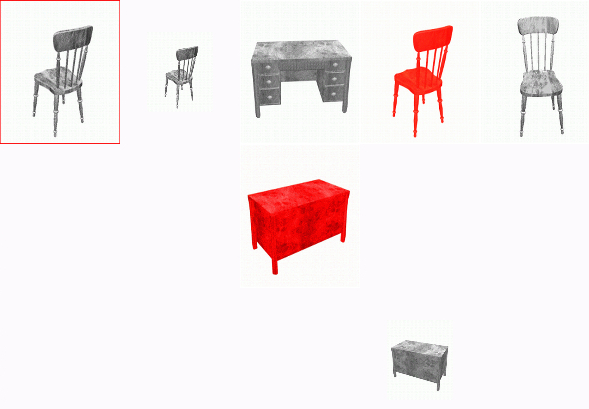
\includegraphics[width=\textwidth]{images/largeGreyChair.jpg}\\[0pt]
\caption{Imagen del TUNA corpus (muebles)}
\label{fig-TUNA-furniture}
\vspace*{.1cm}
\end{minipage}
\hspace*{0cm}
\begin{minipage}[t]{0.5\linewidth}
\centering
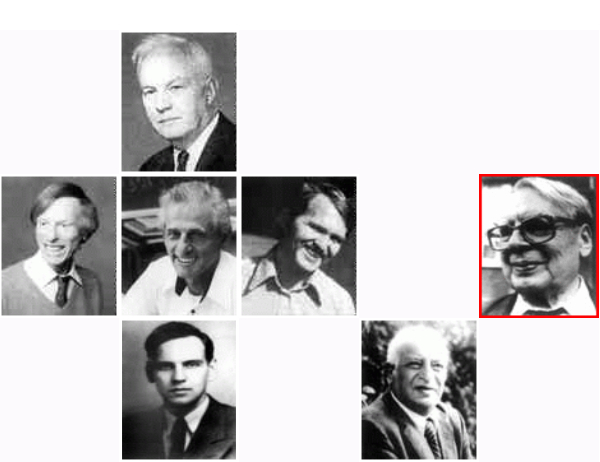
\includegraphics[width=\textwidth]{images/tuna-people.jpg}\\[0pt]
\caption{Imagen del TUNA corpus (personas)}
\label{fig-TUNA-people}
\end{minipage}
\end{figure}


\label{sec:corpusGRE}
%were developed in a series of web-based experiments primarily focussed on the study of relational descriptions. GRE3D3 contains 630 descriptions produced by 63 speakers, and GRE3D7 contains 4480 descriptions produced by 287 speakers, making it the largest of its kind to date. The GRE3D domain consists of simple visual scenes containing only two kinds of objects (boxes and spheres) with limited variation in colour and size. In each scene, there is only one possible spatial relation between target and the nearest landmark. Both corpora contain atomic and relational descriptions.
GRE3D3 y su extensi\'on GRE3D7 \cite{gre3d3,gre3d7} se desarrollaron en una serie de experimentos basados en la web se centraron principalmente en el estudio de las descripciones relacionales. GRE3D3 contiene 630 descripciones producidas por 63 personas y GRE3D7 contiene 4.480 descripciones producidas por 287 personas, y es el corpus m\'as grande de este tipo hasta la fecha. El dominio GRE3D consta de escenas visuales simples que contienen s\'olo dos tipos de objetos (cubos y esferas) con variaci\'on limitada en color y tama\~o. En cada escena, s\'olo hay una posible relaci\'on espacial entre el target y el landmark m\'as cercano. Ambos corpus contienen descripciones at\'omicas y relacionales. Ejemplo de im\'agenes del GRE3D3 y GRE3D7 se muestran en las Figuras \ref{fig-GRE3D3} y \ref{fig-GRE3D7}
%\begin{minipage}[b]{0.45\linewidth}

\begin{figure}
\begin{minipage}[b]{0.5\linewidth}
\centering
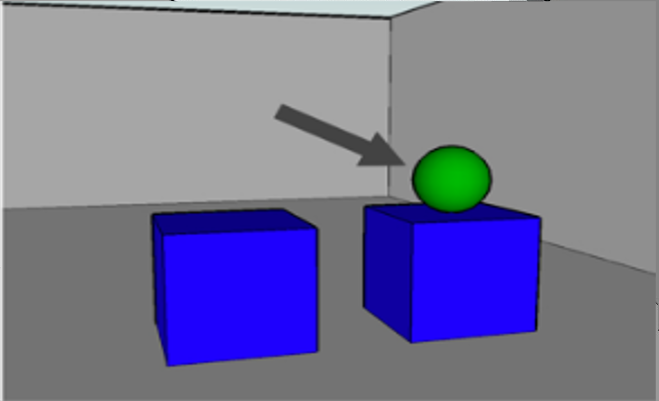
\includegraphics[width=\textwidth]{images/GRE3D3.png}\\[0pt]
\caption{Imagen del GRE3D3}
\label{fig-GRE3D3}
\vspace*{-0.7cm}
\end{minipage}
\hspace*{0cm}
\begin{minipage}[b]{0.5\linewidth}
\centering
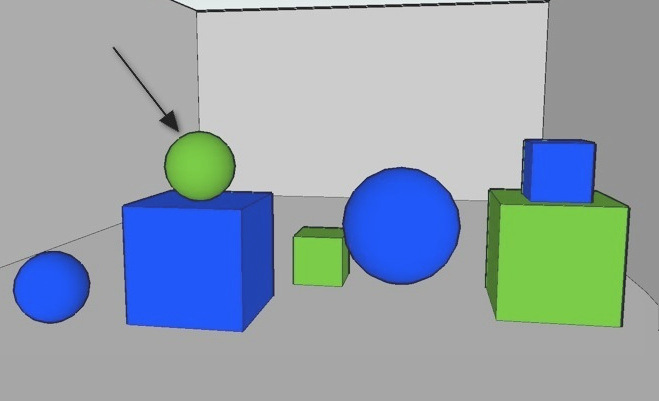
\includegraphics[width=\textwidth]{images/3.jpg}\\[0pt]
\caption{Imagen del GRE3D7}
\label{fig-GRE3D7}
\end{minipage}
\end{figure}

\vspace*{3cm}

\label{sec:corpusSTARS}
%and its extension Stars2 were collected for the study of referential overspecification (particularly in the case of relational descriptions). Stars was developed in a pilot web-based experiment, containing 704 descriptions produced by 64 speakers.  The more comprehensive Stars2 data set was produced in dialogue situations involving subject pairs, and it contains 884 descriptions produced by 56 speakers. Both domains make use of simple visual scenes containing up to four object types (e.g., stars, boxes, cones and spheres) with limited variation in colour and size. Differently from other REG corpora, however, Stars/2 includes a considerable number of complex situations of reference involving up to three objects, as in `the box near the sphere, next to the cone'.http://ppgsi.each.usp.br/arquivos/RelTec/PPgSI-002_2014.pdf y http://ppgsi.each.usp.br/arquivos/RelTec/PPgSI-001_2015.pdf
Stars \cite{stars-mutual-disamb} y su extensi\'on Stars2 se colectaron para el estudio de la sobre-especificaci\'on (particularmente en el caso de las descripciones relacionales). Stars se desarroll\'o en un experimento piloto basado en la web, contiene 704 descripciones producidas por 64 personas. El conjunto de datos Stars2 es m\'as completo y se obtuvo de situaciones de di\'alogo que implicaban a dos personas, contiene 884 descripciones producidas por 56 participantes. Ambos dominios hacen uso de escenas visuales simples que contienen hasta cuatro tipos de objetos (por ejemplo para Stars, estrellas, cuadrados y c\'irculos y para Stars2 cubos, conos y esferas) con variaci\'on limitada en color y tama\~o. A diferencia de otros corpus para GER, Stars/2 incluye un n\'umero considerable de situaciones complejas de referencia en que participan hasta tres objetos, como en ``el cubo cerca de la esfera, al lado del cono''. Ejemplos de imagenes se muestran en las Figuras \ref{fig-STARS} y \ref{fig-STARS2}


\begin{figure}
\begin{minipage}[b]{0.5\linewidth}
\centering
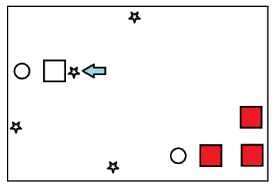
\includegraphics[width=\textwidth]{images/STARS.png}\\[0pt]
\caption{Imagen de Stars corpus}
\label{fig-STARS}
%\vspace*{1cm}
\end{minipage}
\hspace*{0cm}
\begin{minipage}[b]{0.5\linewidth}
\centering
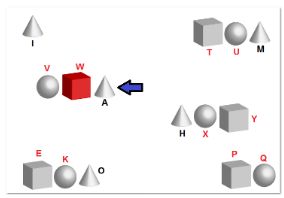
\includegraphics[width=\textwidth]{images/STARS2.png}\\[0pt]
\caption{Imagen de Stars2 corpus}
\label{fig-STARS2}
\end{minipage}
\end{figure}

%ejemplo minipage
%\begin{figure}
%\begin{minipage}[b]{0.5\linewidth}
%\centering
%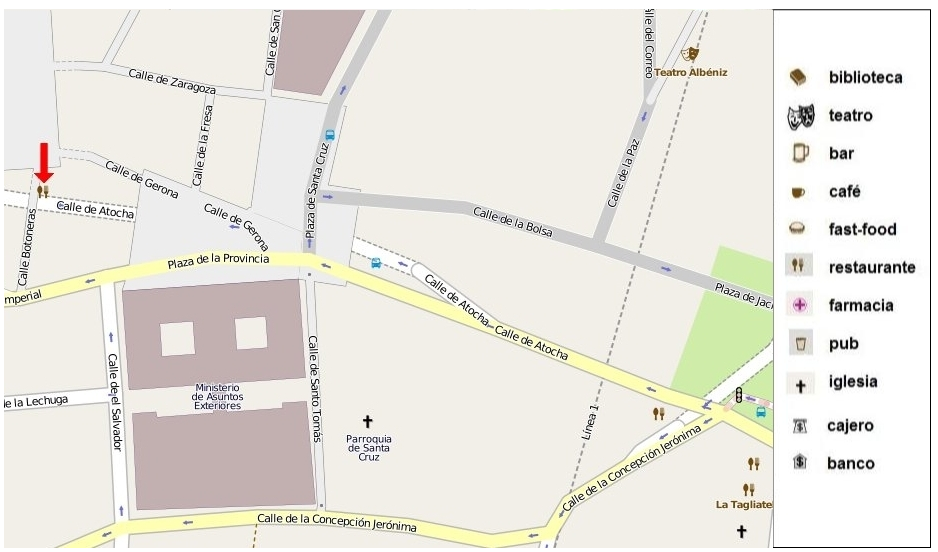
\includegraphics[width=\textwidth]{figures/rest-singular2x.png}\\[0pt]
%\caption{Target singular con zoom 2X}
%\label{rest-singular2x}
%\end{minipage}
%\vspace*{.1cm}
%\begin{minipage}[b]{0.5\linewidth}
%\centering
%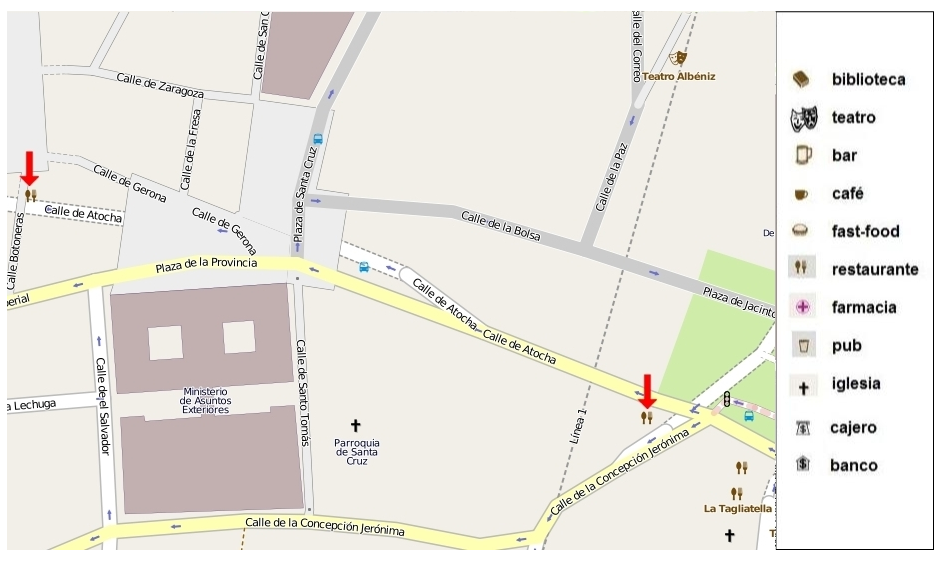
\includegraphics[width=\textwidth]{figures/rest-plural2x.png}\\[0pt]
%\caption{Target plural con zoom 2X}
%\label{rest-plural2x}
%\end{minipage}
%\end{figure}




%Despite their usefulness and general contribution to the research in REG, the above domains are still at a certain distance from the kinds of visual scene that might be required for a practical, real-world application. The need for additional complexity and/or realism, and our own interest in the surface realisation task for the Spanish and Portuguese languages, has led us to build a new computational resource of this kind. This work is described in the next sections. Further discussion on the differences between the Zoom corpus and existing resources is presented in Sec. \ref{sec-annotation}. 



\subsection{Jette y otros trabajos emp\'iricos}

%http://link.springer.com/chapter/10.1007/978-3-642-15573-4_9
%http://www.jetteviethen.net/papers/DaleViethen2010chapter.pdf

La investigaci\'on presentada en \cite{viethen-phd} se basa en dos premisas fundamentales: que la investigaci\'on
en la generaci\'on autom\'atica de expresiones referenciales debe esforzarse por lograr
sistemas que den salidas tan similar a la humana como sea posible; y que, para ello, debemos
esforzarnos para modelar el comportamiento humano como se puede observar en corpora.

La adopci\'on de estas premisas sirve para dos fines: en primer lugar, mejora la adecuaci\'on
de la salida de algoritmos de GER para el objeto target imitando la capacidad humana
de producir referencias adecuadas; y en segundo lugar, el estudio de corpus de datos producidos por humanos
 y algoritmos en desarrollo que pueden replicar estos datos podr\'ian
acercarnos a la comprensi\'on de que es lo que hacen los humanos cuando dan una ER.\\

Se\~nala que el cl\'asico algoritmos de GER y la mayor parte de sus descendientes no se basaron ni evaluaron contra datos producidos por humanos. Ellos se basaron en una visi\'on bastante minimalista de lo que se necesita
para que una expresi\'on referencial sea \'optima, concentr\'andose en la eficiencia computacional 
 y descripciones breves como sus principales preocupaciones.\\

 Existe un peque\~no n\'umero de enfoques que 
 se basaron en observaciones del comportamiento de referencia general humana
que obtuvieron a partir de experimentos psicoling\"u\'isticos, pero de nuevo no fueron evaluados
contra datos humanos.\\

Los algoritmos que se presentaron a los desaf\'ios de evaluaci\'on \cite{gatt-balz-kow:2008:ENLG} y \cite{reg2009}
fueron probados en el TUNA-Corpus, y algunos de ellos
tambi\'en tuvieron en cuenta los patrones que se encontraban en el conjunto del desarrollo. Pero hay una serie de preocupaciones en torno a la pregunta de si el TUNA-Corpus, y la forma de salida de los sistemas que se compar\'o 
en los desaf\'ios eran ideales para una evaluaci\'on de la adecuaci\'on descriptiva de GER.\\
%saque esto porque no se entiende
%A partir de los desaf\'ios que se describen en m\'as detalle y para evaluarlos en una serie de datos m\'as grande
%que contiene m\'as de una expresi\'on referencial para cada elemento est\'imulo.
Aborda tres \'areas principales en las que los corpus se puede utilizar para
promover el objetivo de la semejanza humana en la investigaci\'on sobre generaci\'on de expresiones referenciales:
evaluaci\'on, la recolecci\'on de corpus y an\'alisis y modelizaci\'on estad\'istica de
datos de corpus.\\
Comenz\'o con el an\'alisis del estado del arte de la investigaci\'on en
la generaci\'on de descripciones distintivas, trabaj\'o con las relaciones espaciales y en el trabajo us\'o datos de corpus. Examin\'o una serie de opciones metodol\'ogicas que tienen que hacerse cuando se trabaja con los corpus de GER. Aqu\'i, explor\'o diferentes opciones para los desaf\'ios de recopilaci\'on de corpus, que se centran en torno al equilibrio que se necesita
entre el control de los par\'ametros experimentales tanto como sea necesario
y mantener la configuraci\'on de lo m\'as natural posible. Discuti\'o una serie de conceptos
que son de importancia para el an\'alisis de corpora de GER, tales como la naturalidad de diferentes
propiedades de los objetos, y las nociones de minimalidad y cuestiones de sobre-especificaci\'on de expresiones referenciales. Por \'ultimo, analiz\'o diferentes maneras en que la salida de un sistema se puede
comparar con los datos corpus, bajo la premisa de que el objetivo de la comparaci\'on es
para evaluar si el sistema podr\'ia tener un modelo adecuado del comportamiento humano para la generaci\'on de expresiones referenciales.
Realiz\'o una investigaci\'on en las tres \'areas donde corpora se pueden emplear en GER: Evaluaci\'on de semejanza humana, recopilaci\'on y an\'alisis de corpus, y modelado de datos de corpus. Realiz\'o un experimento de evaluaci\'on en
que tres de los algoritmos cl\'asicos, (1989) Algoritmo Greedy de Dale (Greedy), Dale y Haddock (1991b), Relacional Algoritmo (ra) Y Dale y Reiter (1995) Algoritmo incremental (IA), Se pusieron a prueba en cuanto a su capacidad de
replicar las expresiones referenciales se encuentran en un grupo relativamente peque\~no de corpus de expresiones referenciales
en un dominio visual de im\'agenes puestas en una grilla.
%de rejilla de cajones de armarios ling. 
En el analisis de este experimento tuvo dos resultados principales: (1) que identic\'o en particular tres 
fen\'omenos que todav\'ia plantean importantes retos para los algoritmos GER con el objetivo de replicar
el comportamiento humano, y (2) que proporciona una plataforma para la discusi\'on de una serie de
dificultades que se presentan para la evaluaci\'on basada en corpus de GER. Esto result\'o en una serie
de criterios para el dise\~no de los dos corpus que el trabajo en el resto de la tesis.
Los tres fen\'omenos en las expresiones referenciales producidas por humanos que los
algoritmos probados no fueron capaces de replicar satisfactoriamente eran demasiado espec\'ificas,
relaciones espaciales, y el comportamiento de voluntarios espec\'ificos. Ambos
Greddy y la IA fueron capaz de generar algo de la redundancia que se encontr\'o en el corpus, sino un
n\'umero de las expresiones referenciales conten\'ia informaci\'on m\'as redundante que
ya sea algoritmo podr\'ia producir bajo cualquier ajuste de par\'ametros, gobernando a cabo como
modelos precisos de referencia comportamiento humano. Ni codicioso ni el Iowa estaban destinados a ser capaz de generar refiri\'endose expresiones que contienen las relaciones entre entidades, pero esto es exactamente lo que el
ra fue dise\~nado. Sorprendentemente, la
ra no s\'olo no para generar cualquiera de las
descripciones contenidas en el corpus de evaluaci\'on; las descripciones que se generan
parec\'ia m\'as como enigmas cuyo objetivo era confundir a un oyente, m\'as que \'util
los intentos de se\~nalar el referente objetivo. Una valoraci\'on te\'orica de otro AP
enfoques dise\~nados para manejar las relaciones establecieron que ninguno de ellos incluir\'ia
una relaci\'on en el dominio de prueba, porque una relaci\'on nunca fue absolutamente necesario
distinguir cualquiera de los cajones.
La tercera \'area de preocupaci\'on que el experimento puso de relieve fue la observaci\'on
que la gente no todos hacen lo mismo en la misma situaci\'on. De hecho, incluso
la misma persona podr\'ia describir el mismo caj\'on de di? erently bajo di? cir- Erent
cunstancias. Ninguno de los algoritmos de prueba se pretende tomar las inter e
variaci\'on intra-hablante en cuenta, y s\'olo muy recientemente han implementaciones
del Iowa comenzado a modelo de altavoz-preferencias en alg\'un grado.
Los temas generales con evaluaci\'on basada en corpus que esta experiencia de evaluaci\'on
ci\'on al descubierto fueron (1) la interdependencia estrecha entre algoritmos y la
representaci\'on subyacente de conocimientos que utilizan, (2) la no-determinismo de natu-
generaci\'on ral lenguaje, (3) la cuesti\'on de c\'omo comparar la salida algoritmos '
a muchas normas de oro, y (4) la ciudad-dominio espec\'ifico de GER algoritmos. La
discusi\'on de estos temas ha dado lugar a la siguiente desiderata de corpus basa-
Evaluaci\'on en GER:

1. Si corpora est\'an destinados para ser reutilizado para la evaluaci\'on comparativa de diferentes
algoritmos, una representaci\'on subyacente del dominio debe ser proporcionado
junto a ellos.
2. Si queremos ser mella acondicionado en ning\'un resultado de la evaluaci\'on basada en un GER
corpus, este corpus debe contener tantos casos como sea posible de tantos direntes altavoces como sea posible para cada escenario referencial. Esto es cierto si
un algoritmo es evaluado en t\'erminos de ser capaz de generar una natural
sonando refiri\'endose expresi\'on, o si est\'a probado por su probabilidad de BE-
ing un modelo preciso de la conducta humana de referencia mediante la comprobaci\'on de si se puede
generar todas las descripciones en un corpus.
3. Si la probabilidad de un algoritmo de ser un modelo de conducta humana de referencia
se eval\'ua, deben utilizarse m\'etricas basadas en recuerdo y la precisi\'on. En esto
caso, el conjunto completo de las descripciones que el algoritmo proporciona para cada
escenario de referencia en virtud de cualquier ajuste de par\'ametro debe ser comparado con el
conjunto de las descripciones contenidas en el corpus para el mismo escenario referencial.
Si la capacidad m\'as orientado a la aplicaci\'on para generar una referencia similar a la humana
se ha de evaluar, s\'olo una descripci\'on por escenario debe ser evaluado.
Esto debe hacerse utilizando una m\'etrica basada en la precisi\'on para probar c\'omo muchos de los
descripciones algoritmos 'est\'an contenidos en el corpus.
4. Algoritmos que son juzgados en un dominio espec\'ifico c no deben ser asumidas como
f\'acilmente adaptable a otros dominios. Idealmente, los corpus que abarca muchos diferentes
deben estar disponibles para las reclamaciones de los algoritmos de prueba tipos de dominios
generalizaci\'on
\subsection{M\'etricas de evaluaci\'on/comparaci\'on con corpus}

Para medir la performance de los algoritmos podemos usar m\'etricas autom\'aticas o m\'etricas manuales, las m\'etricas autom\'aticas son aquellas que se calculan mediante un algoritmo y las manuales en las cuales les requerimos a personas que evaluen las expresiones referenciales.


\subsubsection{M\'etricas autom\'aticas}


La exactitud (Accuracy) se define como el porcentaje de coincidencias exactas entre cada RE producida por un ser humano y la producida por el sistema para la misma escena y target. Se considera que es una m\'etrica demasiado estricta.\\


El coheficiente Dice es una m\'etrica de comparaci\'on de conjuntos, el valor va entre 0 y 1, 1 indica un perfecto match entre los conjuntos. Para dos conjuntos A y B, Dice se calcula como sigue:\\

$Dice(A,B) = \frac{2\times|A \cap B|}{|A|+|B|}$\\

\textsc{masi} de \cite{Passonneau06measuringagreement}~es una adaptaci\'on de el coheficiente Jaccard el cual varia en favor de la similaridad cuando un conjunto es un subconjunto de otro, como Dice varia entre 0 y 1, 1 indica match perfecto. Se calcula como sigue:\\
%which biases it in favor of similarity where one set
%is a subset of the other. Like Dice, it ranges between
%0 and 1, where 1 indicates a perfect match. It is computed as follows:\\

$\textsc{masi}(A,B) = \delta \times \frac{|A \cap B|}{|A \cup B|}$ \\


donde $\delta$ es un coheficiente \textcolor{blue}{``monotonicity'' (NO SE QUE ES)} definido como sigue:\\


 \begin{equation}
     \delta  = \left\{
	       \begin{array}{ll}
		 0      & if A \cap B = \emptyset \\
		 1 & if A = B  \\
		 \frac{2}{3}     & if A \subset B ~or~ B \subset A\\
		 \frac{1}{3}     & otherwise
	       \end{array}
	     \right.
 \end{equation}

Intuitivamente significa que se prefieren aquellas descripciones producidas por el sistema las cuales no incluyen atributos que los humanos no incluyeron.
%Intuitively, this
%means that those system-produced descriptions are
%preferred which do not include attributes that are
%omitted by a human.  

\subsubsection{M\'etricas manuales}
